\chapter{Descrição dos Módulos}

A arquitetura da aplicação a desenvolver é definida por quatro módulos principais: Catálogo de clientes, Catálogo de produtos, Faturação Global e Vendas por Filial, cujas fontes de dados são três ficheiros de texto detalhados abaixo.
 
\paragraph{}
No ficheiro \textbf{Produtos.txt} cada linha representa o código de um produto vendável no hipermercado, sendo cada código formado por duas letras maiúsculas e 4 dígitos (que representam um inteiro entre 1000 e 1999), como no exemplo: 

\begin{verbatim}
AB9012
XY1185
BC9190
\end{verbatim}

O ficheiro de produtos contém cerca de 200.000 códigos de produto. 

\paragraph{}
No ficheiro \textbf{Clientes.txt} cada linha representa o código de um cliente identificado no hipermercado, sendo cada código de cliente formado por uma letra maiúscula e 4 dígitos que representam um inteiro entre 1000 e 5000, segue um exemplo: 

\begin{Verbatim}
F2916
W1219
F2915
\end{Verbatim}

O ficheiro de clientes contém cerca de 20.000 códigos de cliente. 

\paragraph{}
O ficheiro \textbf{Vendas\_1M.txt}, no qual cada linha representa o registo de uma venda efectuada numa qualquer das 3 filiais da Cadeia de Distribuição. Cada linha (a que chamaremos compra ou venda, o que apenas depende do ponto de vista) será formada por um código de produto, um preço unitário decimal (entre 0.0 e 999.99), o número inteiro de unidades compradas (entre 1 e 200), a letra \textbf{N} ou \textbf{P} conforme tenha sido uma compra \textbf{Normal} ou uma compra em \textbf{Promoção}, o código do cliente, o mês da compra (1 .. 12) e a filial (de 1 a 3) onde a venda foi realizada, como se pode verificar nos exemplos seguintes:
 
 \begin{Verbatim}
KR1583 77.72 128 P L4891 2 1
QQ1041 536.53 194 P X4054 12 3
OP1244 481.43 67 P Q3869 9 1
JP1982 343.2 168 N T1805 10 2
IZ1636 923.72 193 P T2220 4 2 
 \end{Verbatim}
 
 
O ficheiro de vendas inicial, \textbf{Vendas\_1M.txt} , conterá 1.000.000 (1 milhão) de registos de vendas realizadas nas 3 filiais da cadeia de distribuição. 
 
\paragraph{}
A aplicação possuiu uma arquitectura tal como apresentado na figura seguinte, em que se identificam as fontes de dados, a sua leitura e os módulos de dados a construir: 

\begin{figure}  
	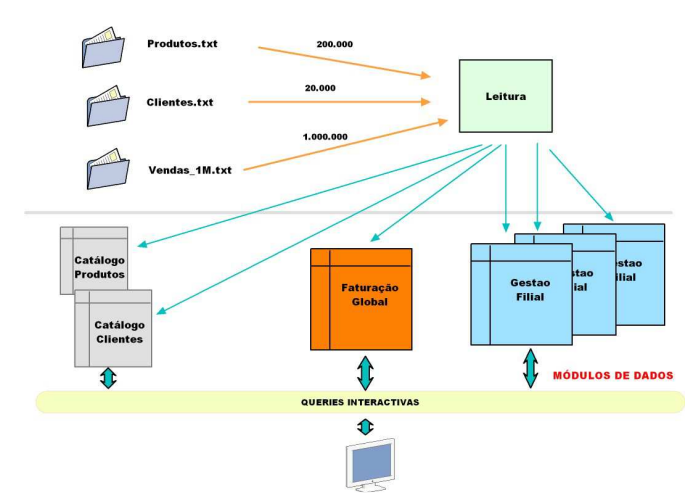
\includegraphics[scale=0.8]{arquiteturaproj.png}  
	\caption{Arquitetura da aplicação}  
\end{figure}



\section{Catálogo de Clientes}
É o módulo de dados onde são guardados os códigos de todos os clientes do ficheiro \textbf{Clientes.txt}, organizados por índice alfabético; 

\subsection{Clientes.h}
\subsubsection{Tipos Opacos}

\begin{Verbatim}
typedef struct catalogo_clientes *CatClientes;
\end{Verbatim}


\begin{Verbatim}
CatClientes inicializa_catalogo_clientes();
void insertC(CatClientes c, char * valor);
void cat_remove_cliente(CatClientes cat, char *str);
void free_catalogo_Clientes(CatClientes cat);
int existeCliente (char *cliente,CatClientes cat);
int numeroClientes(CatClientes cat);
int numeroClientesLetra(CatClientes cat, char letra);
\end{Verbatim}

\section{Catálogo de Produtos}

 Módulo de dados onde são guardados os códigos de todos os produtos do ficheiro \textbf{Produtos.txt}, organizados por índice alfabético, o que irá permitir, de forma eficaz, saber quais são os produtos cujos códigos começam por uma dada letra do alfabeto, quantos são



\subsection{Produtos.h}

\subsubsection{Tipos Opacos}
\begin{verbatim}
typedef struct catalogo_produtos *CatProdutos;
\end{verbatim}


\begin{Verbatim}
CatProdutos inicializa_catalogo_produtos();
void insertP(CatProdutos c, char * valor);
void cat_remove_produto(CatProdutos cat, char *str);
void free_catalogo_produtos(CatProdutos cat);
int existeProduto (char *produto,CatProdutos cat);
int numeroProdutos(CatProdutos cat);
int numeroProdutosLetra(CatProdutos cat, char letra);
ARRAY listaProdutosLetra(CatProdutos cat, char l);
\end{Verbatim}


\section{Faturação Global}

Módulo de dados que contém as estruturas de dados responsáveis pela resposta eficiente a questões quantitativas que relacionam os produtos às suas vendas mensais, em modo Normal (N) ou em Promoção (P), para cada um dos casos guardando o número de vendas e o valor total de faturação de cada um destes tipos. Este módulo deve referenciar todos os produtos, mesmo os que nunca foram vendidos.
Este módulo não contém qualquer referência a clientes, mas deve ser capaz de distinguir os valores obtidos em cada filial; 

\subsection{Produtos.h}

\subsubsection{Tipos Opacos}
\begin{Verbatim}
typedef struct faturacao *Faturacao;
typedef struct info *Info;
\end{Verbatim}

\section{Gestão da Filial}


Módulo de dados que, a partir dos ficheiros lidos, contém as estruturas de dados adequadas à representação dos relacionamentos, fundamentais para a aplicação, entre produtos e clientes, ou seja, para cada produto, saber quais os clientes que o compraram, quantas unidades cada um comprou, em que mês e em que filial. Para a estruturação optimizada dos dados deste módulo de dados será crucial analisar as queries que a aplicação deverá implementar, tendo sempre em atenção que pretendemos ter o histórico de vendas organizado por filiais para uma melhor análise, não esquecendo que existem 3 filiais nesta cadeia. 

\subsection{Filial.h}

\subsubsection{Tipos Opacos}
\begin{Verbatim}
typedef struct filial *Filial;
typedef struct icliente *Icliente;
typedef struct iprodutos *Iprodutos;
\end{Verbatim}


\chapter{Main.c}

\chapter{Interface do utilizador}

\chapter{Resultados e comentários sobre os testes de performance}

\chapter{Makefile e Grafo de dependências}